%%
%% This is file `docultexmm.tex', 
%% Documentation for siam multimedia macros for use with LaTeX 2e
%% 
%% December 19, 2013
%%
%% Version 1.0.1
%% 
%% You are not allowed to change this file. 
%% 
%% You are allowed to distribute this file under the condition that 
%% it is distributed together with all of the files in the siam macro 
%% distribution. These are:
%%
%%  siamltexmm.cls (this file)
%%  siam11.clo   (required size option for 11pt papers)
%%  subeqn.clo   (allows equation numbers with lettered subelements)
%%  siam.bst     (bibliographic style file for BibTeX)
%%  docultexmm.tex (documentation file)
%%
%% If you receive only some of these files from someone, please contact: 
%% multimedia@siam.org  
%% 
%% You are not allowed to distribute this file alone. You are not 
%% allowed to take money for the distribution or use of either this 
%% file or a changed version, except for a nominal charge for copying 
%% etc.
%%
%% \CharacterTable
%%  {Upper-case    \A\B\C\D\E\F\G\H\I\J\K\L\M\N\O\P\Q\R\S\T\U\V\W\X\Y\Z
%%   Lower-case    \a\b\c\d\e\f\g\h\i\j\k\l\m\n\o\p\q\r\s\t\u\v\w\x\y\z
%%   Digits        \0\1\2\3\4\5\6\7\8\9
%%   Exclamation   \!     Double quote  \"     Hash (number) \#
%%   Dollar        \$     Percent       \%     Ampersand     \&
%%   Acute accent  \'     Left paren    \(     Right paren   \)
%%   Asterisk      \*     Plus          \+     Comma         \,
%%   Minus         \-     Point         \.     Solidus       \/
%%   Colon         \:     Semicolon     \;     Less than     \<
%%   Equals        \=     Greater than  \>     Question mark \?
%%   Commercial at \@     Left bracket  \[     Backslash     \\
%%   Right bracket \]     Circumflex    \^     Underscore    \_
%%   Grave accent  \`     Left brace    \{     Vertical bar  \|
%%   Right brace   \}     Tilde         \~}

\documentclass[final,leqno,onefignum,onetabnum]{siamltexmm}

\usepackage{amsmath}
\usepackage{amsfonts}

\usepackage{epsfig}


\title{Data-driven Reduction of Multiscale Stochastic Dynamical Systems \thanks{This work was
supported by ....}} 

\author{Carmeline J. Dsilva\footnotemark[2] \and Ronen Talmon\footnotemark[3] \and C. William Gear\footnotemark[2] \and Ronald R. Coifman\footnotemark[3] \and Ioannis G. Kevrekidis\footnotemark[2]\ \footnotemark[4]}

\begin{document}
\maketitle
\newcommand{\slugmaster}{%
\slugger{siads}{xxxx}{xx}{x}{x--x}}%slugger should be set to juq, siads, sifin, or siims

\renewcommand{\thefootnote}{\fnsymbol{footnote}}

\footnotetext[2]{Department of Chemical and Biological Engineering, Princeton University, Princeton, New Jersey, 08544, USA}
\footnotetext[3]{Department of Mathematics, Yale University, New Haven, Connecticut, 06520, USA}
\footnotetext[4]{Program in Applied and Computational Mathematics, Princeton University, Princeton, New Jersey, 08544, USA}

\renewcommand{\thefootnote}{\arabic{footnote}}

\begin{abstract}

\end{abstract}

\begin{keywords}\end{keywords}

\begin{AMS}
37M10, 62-07
\end{AMS}

\pagestyle{myheadings}
\thispagestyle{plain}
\markboth{C.~J. DSILVA {\it ET AL}}{DATA-DRIVEN REDUCTION OF SDES}


\section{Introduction}

\begin{itemize}

\item
Bridge/connect between data mining/analysis and dynamical systems

\begin{itemize}

\item
Main idea and scope: analyze stochastic dynamical systems using data-driven methods.

\begin{itemize}

\item
Reduction in fast-slow systems using manifold learning

\end{itemize}

\end{itemize}
\item
We cannot use off-the-shelf data-driven methods because they are typically based on metrics and geometry and are not informed (take into account) the dynamics and time.

\item
Our contribution:

\begin{itemize}

\item
We show how to use data analysis methods that are typically applied to data sets for analyzing data collected as a time series from a dynamical system. In particular, we ``propose" a data-driven (graph-based) method for recovering the slow variable of reducible systems.

\item
The method is based mostly on local analysis that combines geometry and dynamics.

\item
We offer rigorous analysis for the method that gives the conditions (for our method to successfully recover the ``right" slow variables), intuition.

\end{itemize}

\end{itemize}

\subsection{Multiscale SDEs}

We consider the following two-scale SDE. 
\begin{equation} \label{eq:general_SDE}
\begin{aligned}
dx_i &= a_i(x_1, \dots, x_n) dt + dW_i, \: 1 \le i \le m \\
dx_i &= -\frac{a_i(x_1, \dots, x_n)}{\epsilon} dt + \frac{1}{\sqrt{\epsilon}} dW_i , \: m+1 \le i \le n
\end{aligned}
\end{equation}
where $W_i$ are independent Brownian motions, and $\epsilon \ll 1$.
%
Therefore, \eqref{eq:general_SDE} defines an $n$-dimensional stochastic system with $m$ slow variables and $n-m$ fast variables. 
%
We would like to note that the ratio of the drift and diffusion terms is essential.
%
We need the square of the diffusivity to be of the same order as the drift.
%
If the diffusivity is too large, the equilibrium measure will be unbounded.
%
Conversely, if the diffusivity is too small, the equilibrium measure will go to 0.

Assuming that the functions $a_i$ are bounded and Lipschitz, and we can find
\begin{equation}
\mathbb{E} \left| \frac{1}{T} \int_t^{t + T} a_i(x_1, \dots, x_m, X_{m+1}(s), \dots, X_n(s)) ds - \overline{a} (x_1, \dots, x_m) \right| < \kappa_i (T) 
\end{equation}
for $1 \le i \le m$, where $\kappa_i((T) \rightarrow 0 $ as $T \rightarrow \infty$, then the averaging principle \cite{...} states that we can write an effective equation in the slow variables $x_1, \dots, x_m$. 
%
We will consider systems that can be written as deterministic (perhaps nonlinear) bi-Lipshitz functions $\mathbf{f}: \mathbb{R}^n \mapsto \mathbb{R}^d$ of the SDE in \eqref{eq:general_SDE}.
%
Our goal is to recover the slow variables $x_1, \dots, x_m$ using data-driven techniques. 

For illustrative purposes, we will consider the following two-dimensional SDE as a specific example of \eqref{eq:general_SDE}. 
\begin{equation} \label{eq:fast_slow_SDE}
\begin{aligned}
dx_1 &= adt + dW_1\\
dx_2 &= -\frac{x_2}{\epsilon} dt + \frac{1}{\sqrt{\epsilon}} dW_2
\end{aligned}
\end{equation}
%
where $a$ is a constant of order 1. 
%
So $x_1$ is the slow variable, and $x_2$ is a fast noise whose equilibrium measure is bounded and $\mathcal{O}(1)$.
%
We would like to recover $x_1$ using data-driven techniques.

We will consider two specific examples. 
%
In the first example, our transformation $\mathbf{f}$ will be the identity function and fast and slow remain uncoupled,
\begin{equation}
\mathbf{f_1}(x_1, x_2) = \begin{bmatrix} x_1 \\ x_2 \end{bmatrix}
\end{equation}

In the second example, our data will be warped into half-moon shapes
\begin{equation}
\mathbf{f_2}(x_1, x_2) = 
\begin{bmatrix} 
x_1 + x_2^2 \\
x_2
\end{bmatrix}
\end{equation}
% 
We will show in both cases how we can recover the slow variables using data-driven techniques. 

\section{Local Invariant Metrics}

To locally recover the slow variables, we need to build a metric that is invariant to the fast variables. 
%
Typically, this is done by averaging out the fast variables. 
%
We propose to do this using the Mahalanobis distance, which is a local PCA-type approach that inverts the local covariance matrix of the data, thereby creating a space with normalized diffusion terms.
%
It can be shown that the Mahalanobis distance locally approximates: 
\begin{equation} \label{eq:mahalanobis}
\| \mathbf{f}(\Xi_1) - \mathbf{f}(\Xi_2) \|^2_M = \| \Xi_1 - \Xi_2 \|^2_2 + \mathcal{O}(\| \mathbf{f}(\Xi_1) - \mathbf{f}(\Xi_2) \|^4_2)
\end{equation}
where the components of $\Xi$ have uncoupled noise with unit variance,
i.e., the variables $\xi_1, \dots, \xi_n$ are governed by the following SDEs:
\begin{equation} \label{eq:NIV_formulation}
d\xi_i = b(\xi) dt + dW_i
\end{equation}
and $\Xi = \begin{bmatrix} \xi_1 & \xi_2& \cdots & \xi_n \end{bmatrix}^T$.

In particular, for SDEs of the form in \eqref{eq:general_SDE}, consider the transformation
\begin{equation} \label{eq:general_rescale}
\begin{aligned}
x_i = \xi_i, \: &1 \le i \le m \\
x_i = \frac{\xi_i}{\sqrt{\epsilon}} \: &1 \le i \le m
\end{aligned}
\end{equation}

Then, \eqref{eq:general_SDE} becomes
\begin{equation} 
\begin{aligned}
d\xi_i &= b_i(\xi_1, \dots, \xi_n) dt + dW_i, \: 1 \le i \le m \\
d\xi_i &= -\frac{b_i(\xi_1, \dots, \xi_n)}{\sqrt{\epsilon}} dt + dW_i , \: m+1 \le i \le n
\end{aligned}
\end{equation}
where $b_i(\xi_1, \dots, \xi_n) = a_i (\xi_1, \dots, \xi_m, \frac{\xi_{m+1}}{\sqrt{\epsilon}}, \dots, \frac{\xi_n}{\sqrt{\epsilon}})$.
%
From \eqref{eq:general_rescale}, we can see that if $x_i = \mathcal{O}(1)$, then $\xi_i = \mathcal{O}({\sqrt{\epsilon}})$ for $ m+1 \le i \le n$, and 
\begin{equation}
\| \Xi_2 - \Xi_1 \|^2_2 = \sum_{i=1}^m \| \xi_{2,i} - \xi_{1,i} \|^2 = \sum_{i=1}^m \|x_{2,i} - x_{1,i} \|^2 + \epsilon \sum_{i=m+1}^n \|x_{2,i} - x_{1,i}\|^2
\end{equation}
%
Remarkably, this metric induces two important features. 
%
One, rescaling the data so that all variables have unit diffusion terms means that fast variables are collapsed and become ``epsilon" small, as observed in the second term in the right hand side. 
%
Two, the righthandside of \eqref{eq:mahalanobis} is invariant (to fourth order) to the function $\mathbf{f}$ and allows for the approximation of the Euclidean distance between samples of the slow variables in the ``decoupled" SDE space.


For the specific example \eqref{eq:fast_slow_SDE}, the change of variables gives the following system:
\begin{equation}
\begin{aligned}
d\xi_1 &= adt + dW_1\\
d\xi_2 &= -\frac{\xi}{\epsilon} dt +  dW_2
\end{aligned}
\end{equation}


\section{Diffusion Maps for Global Parameterization}

Our goal is to extract a {\em global} parameterization of the data that respects the slow variables. 
%
We will use diffusion maps, a kernel-based manifold learning technique, to extract a global parameterization using the local distances that we described in the previous section. 
%
Given data $z_1, \dots, z_N \in \mathbb{R}^d$, we first construct the matrix $W \in \mathbb{R}^{N \times N}$, where 
\begin{equation}
W_{ij} = \exp \left( -\frac{\|z_i - z_j \|^2}{\sigma_{kernel}^2} \right)
\end{equation}
where $\| \cdot \|$ denotes the appropriate norm, and $\sigma_{kernel}$ is the kernel scale and denotes a characteristic distance within the data set (we often set $\sigma_{kernel}$ to be the median of the pairwise distances). 
%
In our applications, we will use the Mahalanobis distance \eqref{eq:mahalanobis} as the norm between points, so that we can recover the slow variables. 

We then construct the diagonal matrix $D \in \mathbb{R}^{N \times N}$, with 
\begin{equation}
D_{ii} = \sum_{j=1}^N W_{ij}
\end{equation}
%
We compute the eigenvalues $\lambda_0, \dots, \lambda_{N-1}$ and eigenvalues $\phi_0, \dots, \phi_{N-1}$ of the matrix $A = D^{-1}W$, and order them such that $|\lambda_0| \ge |\lambda_1| \ge \dots \ge |\lambda_{N-1}|$. 
%
$\phi_0$ is a constant trivial eigenvector; the next few eigenvectors give a parameterization/embedding coordinates for the data. 

\section{Analysis}

\begin{figure}
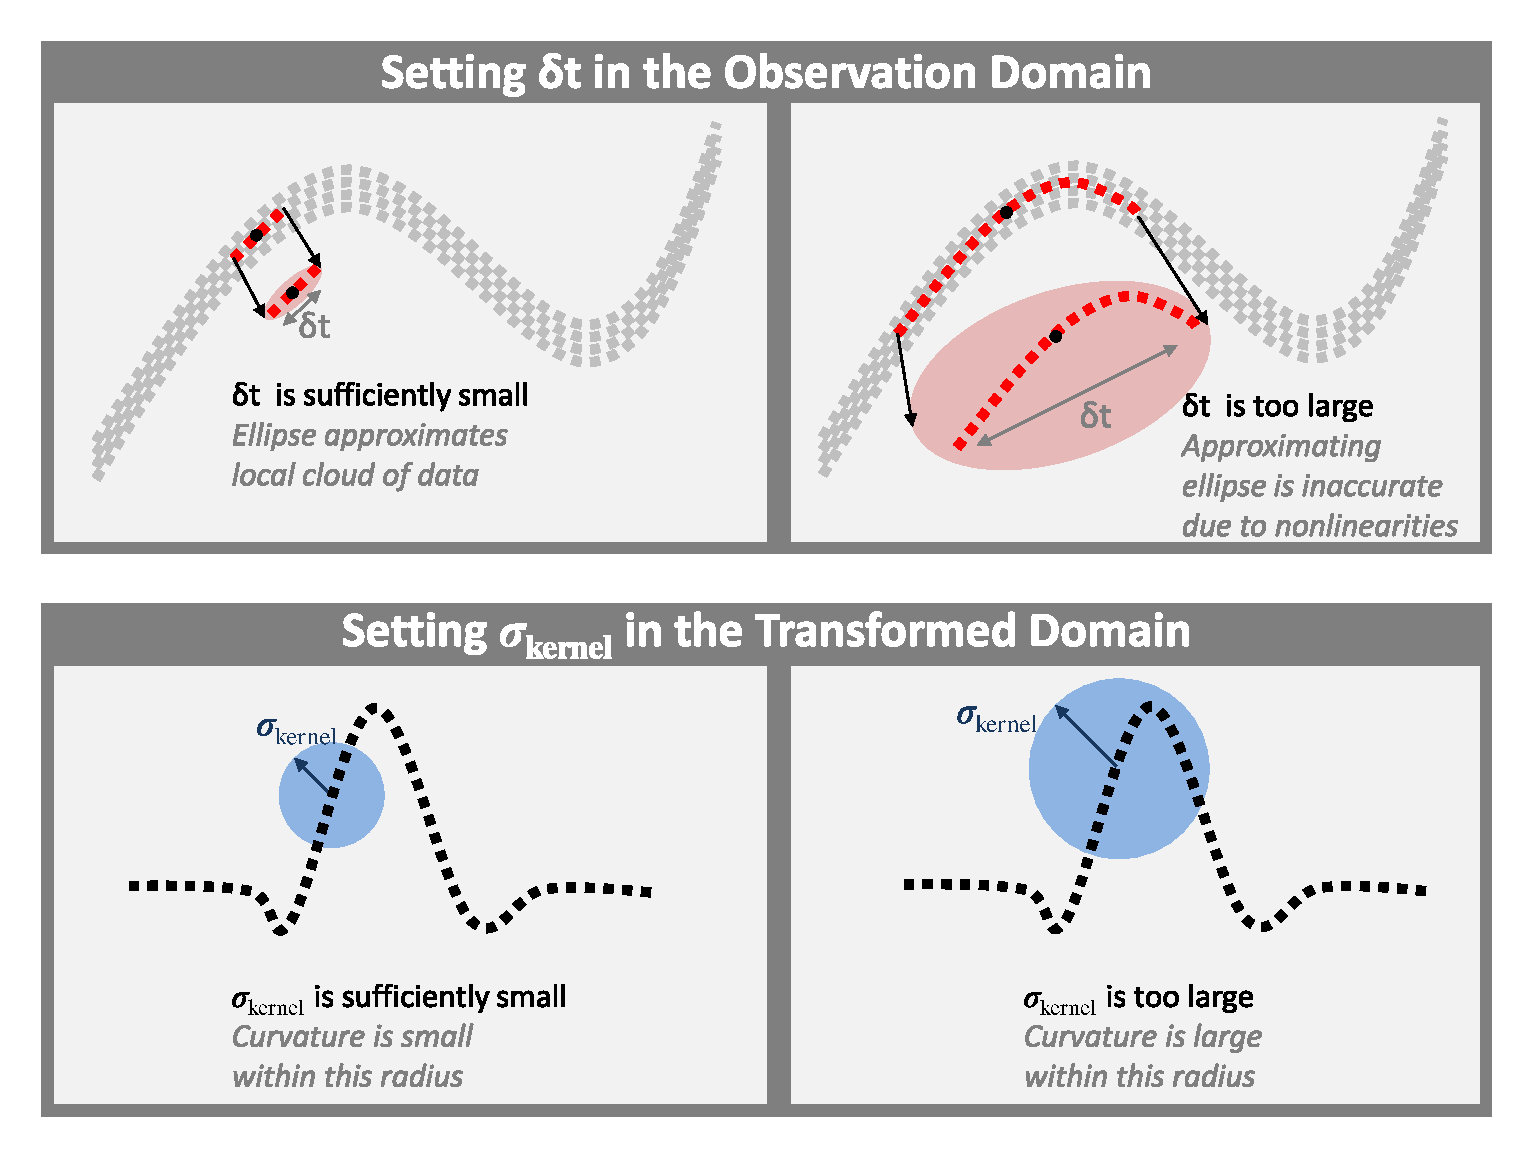
\epsfig{width=\textwidth, file=schematic.eps}
\caption{Illustration of how to choose $\delta t$ and $\sigma_{kernel}$ appropriately. The data shows the evolution of the ``fast'' variable at a fixed value of the ``slow'' variable.  We must choose both parameters so that the curvature effects and other nonlinearities are negligable. }
\label{fig:schematic}
\end{figure}

Our approximation of the pairwise distances will rely on the Taylor expansion of the measurement function $f$. 
%
We will then {\em empirically} estimate the first-order term in this expansion using simulation bursts to estimate the local covariance.  
%
Accordingly, we will address the accuracy of our method from two standpoints: (1) the accuracy of the Taylor expansion, and (2) the accuracy of the covariance estimation (see Figure~\ref{fig:schematic}).
%
We will present both analytical results for the error bounds, as well as an empirical methodology to set the appropriate parameters for our method to accurately recover the intrinsic slow variable(s). 

TODO: change ``curvature'' in figure to ``nonlinearity'' in $\sigma_{kernel}$
TODO: emphasize that if $\delta t$ is too large, then data does not look Gaussian
TODO: change strip to look different than other data


\subsection{Error analysis of the Mahalanobis distance}

Given the true covariance, we can write the Euclidean distance $\|X_2 - X_1 \|$ using Taylor expansion as...

Talk about fourth-order error terms, say we want to choose the kernel scale such that these error terms are negligible. 
%
The error terms involve curvature of $f$, etc.


Let $\mathbf{g} = \mathbf{f}^{-1}: \mathbb{R}^d \mapsto \mathbb{R}^n$, and let $Y_1 = f(X_1)$, and $Y_2 = f(X_2)$.
%
Again, we let $g_j^i = \frac{\partial g^i}{\partial Y^j}$.
%
Then, by Taylor expansion, we obtain
\begin{equation}
\begin{aligned}
x_{2,i} &=& 
x_{1,i} 
+ \sum_{j=1}^d \left. \frac{\partial g_i}{\partial y_j} \right|_{Y_1} (y_{2,j} - y_{1,j} ) 
+ \frac{1}{2} \sum_{j=1}^d \sum_{k=1}^d \left. \frac{\partial^2 g_i}{\partial y_j \partial y_k} \right|_{Y_1} (y_{2,j} - y_{1,j}) (y_{2,k} - y_{1,k}) \\
&&+ \frac{1}{6} \sum_{j=1}^d \sum_{k=1}^d \sum_{l=1}^d \left. \frac{\partial^3 g_i}{\partial y_j \partial y_k \partial y_l} \right|_{Y_1} (y_{2,j} - y_{1,j}) (y_{2,k} - y_{1,k}) (y_{2,l} - y_{1,l})
+ \mathcal{O}( \|Y_2 - Y_1\|^4 )
\end{aligned}
\end{equation}

Substituting the Taylor expansion into the quadratic form, we obtain
\begin{equation}
\begin{aligned}
\| X_2 - X_1 \|^2_2 
=& \frac{1}{2} (Y_2 - Y_1 )^T \left(\left.(J J^T)^{-1}\right|_{Y_1} + \left.(J J^T)^{-1}\right|_{Y_2}\right) (Y_2 - Y_1 ) \\
& + \frac{1}{2} \sum_{i=1}^n \sum_{jkl=1}^{d} \left( \left. \frac{\partial g_i}{\partial y_j} \right|_{Y_1} \left. \frac{\partial^2 g_i}{\partial y_k \partial y_l} \right|_{Y_1} - \left. \frac{\partial g_i}{\partial y_j} \right|_{Y_2} \left. \frac{\partial^2 g_i}{\partial y_k \partial y_l} \right|_{Y_2} \right) (y_{2,j} - y_{1,j})  (y_{2,k} - y_{1,k})(y_{2,l} - y_{1,l}) \\
& + \frac{1}{8} \sum_{i=1}^n \sum_{jklm=1}^d  \left( \left. \frac{\partial^2 g_i}{\partial y_j \partial y_k} \right|_{Y_1} \left. \frac{\partial^2 g_i}{\partial y_l \partial y_m} \right|_{Y_1} + \left. \frac{\partial^2 g_i}{\partial y_j \partial y_k} \right|_{Y_2} \left. \frac{\partial^2 g_i}{\partial y_l \partial y_m} \right|_{Y_2} \right) (y_{2,j} - y_{1,j})  (y_{2,k} - y_{1,k})(y_{2,l} - y_{1,l})(y_{2,m} - y_{1,m}) \\
& + \frac{1}{6}  \sum_{i=1}^n \sum_{jklm=1}^d  \left( \left. \frac{\partial g_i}{\partial y_j} \right|_{Y_1} \left. \frac{\partial^3 g_i}{ \partial y_k \partial y_l \partial y_m} \right|_{Y_1} + \left. \frac{\partial g_i}{\partial y_j} \right|_{Y_2} \left. \frac{\partial^3 g_i}{ \partial y_k \partial y_l \partial y_m} \right|_{Y_2} \right) (y_{2,j} - y_{1,j})  (y_{2,k} - y_{1,k})(y_{2,l} - y_{1,l})(y_{2,m} - y_{1,m}) \\
& + \mathcal{O} (\|Y_1 - Y_2 \|^6 ) 
\end{aligned}
\end{equation}

In general, we do not have access to $f$, $g$, or any of its derivatives.
%
However, we note that $J J^T(Y_1)$ is the local covariance of $Y_1$, which we can empirically estimate from data (this will be discussed in a subsequent section).
%
Therefore, we choose to truncate the distance approximation at the first order term.
%
We call this distance the {\em Mahalanobis distance}, 
\begin{equation}
 \| Y_2 - Y_1 \|^2_M = \frac{1}{2} (Y_2 - Y_1 )^T \left(\left.(J J^T)^{-1}\right|_{Y_1} + \left.(J J^T)^{-1}\right|_{Y_2}\right) (Y_2 - Y_1 )
\end{equation}
%
The error in the approximation is defined as
\begin{equation}
e_M(Y_1, Y_2) = \| X_2 - X_1 \|^2_2 - \| Y_2 - Y_1 \|^2_M 
\end{equation}

We can bound the error by
\begin{equation}
| e_M(Y_1, Y_2)  | \le n \left( \left| K_1 K_2 \right| + \left| \frac{ K_2^2}{4} \right|  + \left| \frac{K_1 K_3}{3} \right|  \right) \| Y_2 - Y_1 \| ^4  
+ \mathcal{O} (\|Y_1 - Y_2 \|^6 ) 
\end{equation}
%
where
%
\begin{equation}
\begin{aligned}
K_1 &= \sup_{i,j,Y} |g_j^i(Y)|\\
K_2 &= \sup_{i,j,k,Y} |g_{jk}^i(Y)|\\
K_3 &= \sup_{i,j,k,l,Y} |g_{jkl}^i(Y)|
\end{aligned}
\end{equation}



\subsection{Error analysis of the covariance estimation}

To compute the Mahalanobis distance, we require $J J^T$. 
%
From \cite{...}, we know that $JJ^T = C$, where $C$ is the local covariance of the observed stochastic process. 
%
Therefore, we would like to estimate the local covariance at a point $X_t$. 

We know that, for a stochastic process following \eqref{eq:general_SDE} and observed through a function $\mathbf{f}$, the covariance $C$ is given by 
\begin{equation}
C_{jk}(X_t) = 
\sum_{i=1}^m \left. \frac{\partial f_j}{\partial x_i} \right|_{X_t} \left. \frac{\partial f_k}{\partial x_i} \right|_{X_t} 
+ \frac{1}{\epsilon} \sum_{i=m+1}^n \left. \frac{\partial f_j}{\partial x_i} \right|_{X_t} \left. \frac{\partial f_k}{\partial x_i} \right|_{X_t} 
\end{equation}

We will use local simulation bursts to estimate the local covariance.
%
Let $X_\tau$ denote the samples at time $\tau > t$. 
%
For the general SDE formulation outlined in \eqref{eq:general_SDE}, we write the estimated covariance $\hat{C}$ as
\begin{equation}
\begin{aligned}
\hat{C}_{jk} (X_t, \tau - t) = & 
\frac{1}{\tau - t} \left(  \mathbb{E} \left[ f_j(X_\tau) f_k(X_\tau) \right] - \mathbb{E}[f_j(X_\tau)]\mathbb{E}[f_k(X_\tau)]   \right)\\
= & \sum_{i=1}^m \left. \frac{\partial f_j}{\partial x_i} \right|_{X_t} \left. \frac{\partial f_k}{\partial x_i} \right|_{X_t}  \\
& + \frac{1}{\epsilon} \sum_{i=m+1}^n \left. \frac{\partial f_j}{\partial x_i} \right|_{X_t} \left. \frac{\partial f_k}{\partial x_i} \right|_{X_t} \\
& + \frac{1}{\tau - t} \sum_{i=1}^m \left. \frac{\partial f_j}{\partial x_i} \right|_{X_t} \mathbb{E} \left[ \left( \int_t^\tau dW_s^i  \right) \left( \int_t^\tau \int_t^{s_2} \frac{\partial^2 f_k}{\partial x_i^2} dW_{s_1}^i dW_{s_2}^i  \right) \right] \\
& + \frac{1}{\epsilon^{3/2} (\tau - t)} \sum_{i=m+1}^n \left. \frac{\partial f_j}{\partial x_i} \right|_{X_t} \mathbb{E} \left[ \left( \int_t^\tau dW_s^i  \right) \left( \int_t^\tau \int_t^{s_2} \frac{\partial^2 f_k}{\partial x_i^2} dW_{s_1}^i dW_{s_2}^i  \right) \right] \\
& + \frac{1}{\tau - t} \sum_{i=1}^m \left. \frac{\partial f_k}{\partial x_i} \right|_{X_t}  \mathbb{E} \left[ \left( \int_t^\tau dW_s^i \right)  \left( \int_t^\tau \int_t^{s_2} \frac{\partial^2 f_j}{\partial x_i^2}  dW_{s_1}^i dW_{s_2}^i \right) \right] \\
& + \frac{1}{\epsilon^{3/2} (\tau - t)} \sum_{i=m+1}^n \left. \frac{\partial f_k}{\partial x_i} \right|_{X_t}  \mathbb{E} \left[ \left( \int_t^\tau dW_s^i \right)  \left( \int_t^\tau \int_t^{s_2} \frac{\partial^2 f_j}{\partial x_i^2}  dW_{s_1}^i dW_{s_2}^i \right) \right] \\
&+ \mathcal{O} ((\tau - t) ) 
\end{aligned}
\end{equation}
%
However, for the specific case when $\mathbf{f}$ is linear, the $\mathcal{O}((\tau - t)^{3/2})$ terms go to 0, and we must consider higher-order terms. 
%
In this case, 
\begin{equation}
\begin{aligned}
\hat{C}_{jk} (X_t, \tau - t) = & 
\frac{1}{\tau - t} \left(  \mathbb{E} \left[ f_j(X_\tau) f_k(X_\tau) \right] - \mathbb{E}[f_j(X_\tau)]\mathbb{E}[f_k(X_\tau)]   \right)\\
= & \sum_{i=1}^m \left. \frac{\partial f_j}{\partial x_i} \right|_{X_t} \left. \frac{\partial f_k}{\partial x_i} \right|_{X_t}  \\
& + \frac{1}{\epsilon} \sum_{i=m+1}^n \left. \frac{\partial f_j}{\partial x_i} \right|_{X_t} \left. \frac{\partial f_k}{\partial x_i} \right|_{X_t} \\
 & + \frac{1}{\tau - t} \sum_{i=1}^m \left. \frac{\partial f_j}{\partial x_i} \right|_{X_t}  \mathbb{E} \left[ \left(\int_t^\tau dW_s^i \right)  \left(\int_t^\tau \int_{t}^{s_2} \left(  \sum_{l=1}^m \frac{\partial a_l}{\partial x_i} \frac{\partial f_k}{\partial x_l}  + \frac{1}{\epsilon} \sum_{l=m+1}^m \frac{\partial a_l}{\partial x_i} \frac{\partial f_k}{\partial x_l} \right)  dW_{s_1}^i ds_2 \right) \right] \\ 
 & + \frac{1}{\epsilon (\tau - t)} \sum_{i=m+1}^n \left. \frac{\partial f_j}{\partial x_i} \right|_{X_t}  \mathbb{E} \left[ \left(\int_t^\tau dW_s^i \right)  \left(\int_t^\tau \int_{t}^{s_2} \left(  \sum_{l=1}^m \frac{\partial a_l}{\partial x_i} \frac{\partial f_k}{\partial x_l}  + \frac{1}{\epsilon} \sum_{l=m+1}^m \frac{\partial a_l }{\partial x_i} \frac{\partial f_k}{\partial x_l} \right)  dW_{s_1}^i ds_2 \right) \right] \\ 
 & + \frac{1}{\tau - t} \sum_{i=1}^m  \left. \frac{\partial f_k}{\partial x_i} \right|_{X_t}  \mathbb{E} \left[ \left(\int_t^\tau dW_s^i \right)  \left(\int_t^\tau \int_{t}^{s_2} \left(  \sum_{l=1}^m \frac{\partial a_l}{\partial x_i} \frac{\partial f_j}{\partial x_l}  + \frac{1}{\epsilon} \sum_{l=m+1}^m \frac{\partial a_l }{\partial x_i} \frac{\partial f_j}{\partial x_l} \right) dW_{s_1}^i ds_2 \right) \right] \\
& + \frac{1}{\epsilon (\tau - t)} \sum_{i=m+1}^n  \left. \frac{\partial f_k}{\partial x_i} \right|_{X_t}  \mathbb{E} \left[ \left(\int_t^\tau dW_s^i \right)  \left(\int_t^\tau \int_{t}^{s_2} \left(  \sum_{l=1}^m \frac{\partial a_l}{\partial x_i} \frac{\partial f_j}{\partial x_l}  + \frac{1}{\epsilon} \sum_{l=m+1}^m \frac{\partial a_l }{\partial x_i} \frac{\partial f_j}{\partial x_l} \right) dW_{s_1}^i ds_2 \right) \right] \\
& + \mathcal{O} ((\tau - t)^{3/2})
 \end{aligned}
\end{equation}
%
For both cases,  we define the error in the estimation as
%
\begin{equation}
\begin{aligned}
e_C (X_t, \tau - t) = \| \hat{C} (X_t, \tau - t)  - C(X_t, \tau - t) \|
\end{aligned}
\end{equation}


\section{Results}


For illustrative purposes, we will consider the following two-dimensional SDE as a specific example of \eqref{eq:general_SDE}. 
\begin{equation}
\begin{aligned}
dx_1 &= adt + dW_1\\
dx_2 &= -\frac{x_2}{\epsilon} dt + \frac{1}{\sqrt{\epsilon}} dW_2
\end{aligned}
\end{equation}
%
where $a$ is a constant of order 1 (we will take $a=3$). 
%
So $x_1$ is the slow variable, and $x_2$ is a fast noise whose equilibrium measure is bounded and $\mathcal{O}(1)$.
%
We would like to recover $x_1$ using data-driven techniques.

\subsection{Linear functions}

In the first example, our transformation $\mathbf{f}$ will be the identity function and fast and slow remain uncoupled,
\begin{equation}
\mathbf{f}(x_1, x_2) = \begin{bmatrix} x_1 \\ x_2 \end{bmatrix}
\end{equation}
%
and
%
\begin{equation}
\mathbf{g}(y_1, y_2) = \mathbf{f}^{-1} (y_1, y_2) = \begin{bmatrix} y_1 \\ y_2 \end{bmatrix}
\end{equation}

In this case, $e_M = 0$, as the second- and higher-order derivatives of $\mathbf{g}$ are all 0. 

\begin{equation}
\begin{aligned}
e_{C, jk} (X_t, \tau - t) = & 
\frac{1}{\tau - t} \sum_{i=1}^m \left. \frac{\partial f_j}{\partial x_i} \right|_{X_t}  \mathbb{E} \left[ \left(\int_t^\tau dW_s^i \right)  \left(\int_t^\tau \int_{t}^{s_2} \left(  \sum_{l=1}^m \frac{\partial a_l}{\partial x_i} \frac{\partial f_k}{\partial x_l}  + \frac{1}{\epsilon} \sum_{l=m+1}^m \frac{\partial a_l}{\partial x_i} \frac{\partial f_k}{\partial x_l} \right)  dW_{s_1}^i ds_2 \right) \right] \\ 
 & + \frac{1}{\epsilon (\tau - t)} \sum_{i=m+1}^n \left. \frac{\partial f_j}{\partial x_i} \right|_{X_t}  \mathbb{E} \left[ \left(\int_t^\tau dW_s^i \right)  \left(\int_t^\tau \int_{t}^{s_2} \left(  \sum_{l=1}^m \frac{\partial a_l}{\partial x_i} \frac{\partial f_k}{\partial x_l}  + \frac{1}{\epsilon} \sum_{l=m+1}^m \frac{\partial a_l }{\partial x_i} \frac{\partial f_k}{\partial x_l} \right)  dW_{s_1}^i ds_2 \right) \right] \\ 
 & + \frac{1}{\tau - t} \sum_{i=1}^m  \left. \frac{\partial f_k}{\partial x_i} \right|_{X_t}  \mathbb{E} \left[ \left(\int_t^\tau dW_s^i \right)  \left(\int_t^\tau \int_{t}^{s_2} \left(  \sum_{l=1}^m \frac{\partial a_l}{\partial x_i} \frac{\partial f_j}{\partial x_l}  + \frac{1}{\epsilon} \sum_{l=m+1}^m \frac{\partial a_l }{\partial x_i} \frac{\partial f_j}{\partial x_l} \right) dW_{s_1}^i ds_2 \right) \right] \\
& + \frac{1}{\epsilon (\tau - t)} \sum_{i=m+1}^n  \left. \frac{\partial f_k}{\partial x_i} \right|_{X_t}  \mathbb{E} \left[ \left(\int_t^\tau dW_s^i \right)  \left(\int_t^\tau \int_{t}^{s_2} \left(  \sum_{l=1}^m \frac{\partial a_l}{\partial x_i} \frac{\partial f_j}{\partial x_l}  + \frac{1}{\epsilon} \sum_{l=m+1}^m \frac{\partial a_l }{\partial x_i} \frac{\partial f_j}{\partial x_l} \right) dW_{s_1}^i ds_2 \right) \right] \\
& + \mathcal{O} ((\tau - t)^{3/2})
 \end{aligned}
\end{equation}

\subsection{Nonlinear functions}

In the second example, our data will be warped into half-moon shapes
\begin{equation}
\mathbf{f_2}(x_1, x_2) = 
\begin{bmatrix} 
x_1 + x_2^2 \\
x_2
\end{bmatrix}
\end{equation}


\begin{itemize}

\item Start with strip: show magnitude of terms, but not figures for terms, because everything will be constant/zero
\item Only error in covariance of strip will be from drift (verify order 1) 
\item Then, show half moons; write error terms explicitly
\item Add drift term to covariance estimation
\end{itemize}


TODO: Also add second example (just strip, no nonlinear transform)


 
Define the following two-dimensional system of SDEs
\begin{eqnarray} \label{eq:init_data}
dX(1) &=& 3 dt + dW_1 \\ 
dX(2) &=& \frac{-X(2)}{\epsilon} dt + dW_2 
\end{eqnarray}
where $W_1, W_2$ are independent Brownian motions, and $\epsilon \ll 1$.
%

Let
\begin{eqnarray}\label{eq:transformed_data}
f^1(X) &=& X(1) + \frac{ X(2)^2}{\epsilon} \\
f^2(X) &=& \frac{X(2)}{\sqrt{\epsilon}}
\end{eqnarray}
Therefore, the two ``intrinsic variables'' $X(1), X(2)$ have been nonlinearly transformed and rescaled such that the new variables $f^1(X), f^2(X)$ are both $\mathcal{O}(1)$, even though $X(1)$ is the ``fast'' variable. 
%
The inverse function $g = f^{-1}$ is
\begin{eqnarray}
g^1(Y) &=& Y(1) - Y(2)^2 \\
g^2(Y) &=& Y(2) \sqrt{\epsilon}
\end{eqnarray}
%
Data from a simulation is shown in Figure~\ref{fig:initial_data}.

%\begin{figure}[h]
%\begin{subfigure}{0.5\textwidth}
%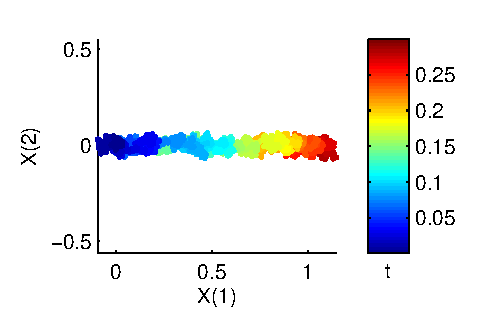
\includegraphics[width=\textwidth]{data_init}
%\caption{}
%\end{subfigure}
%\begin{subfigure}{0.5\textwidth}
%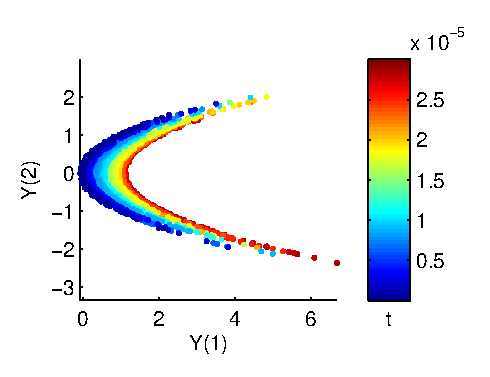
\includegraphics[width=\textwidth]{data_transformed}
%\caption{}
%\end{subfigure}
%\caption{(a) The original data, simulated from \eqref{eq:init_data} with $\epsilon = 10^{-3}$. We take $3000$ timesteps with $dt = 10^{-4}$ (b) The data from (a), transformed according to \eqref{eq:transformed_data}. }
%\label{fig:initial_data}
%\end{figure}

\subsection{NIVs versus DMAPS}

We first want to demonstrate the utility of NIVs over DMAPS. 
%
We compute the first (nontrivial) NIV and DMAPS coordinate using the data in Figure~\ref{fig:initial_data}(b). 
%
The results are shown in Figure~\ref{fig:NIV_versus_DMAPS}.
%
NIV accurately recovers the slow variable (the coloring in Figure~\ref{fig:NIV_versus_DMAPS}(a) is consistent with the coloring in Figure~\ref{fig:initial_data}(b)). 
%
In contrast, DMAPS does not recover the slow variable. 

%\begin{figure}[h]
%\begin{subfigure}{0.5\textwidth}
%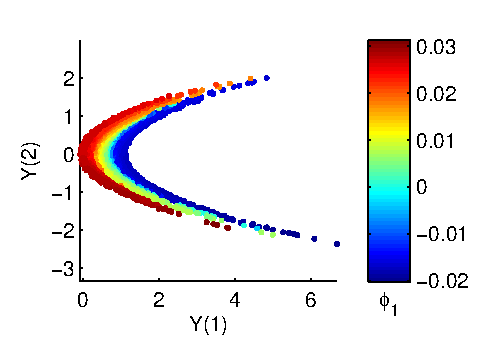
\includegraphics[width=\textwidth]{data_transformed_colored_NIV}
%\caption{}
%\end{subfigure}
%\begin{subfigure}{0.5\textwidth}
%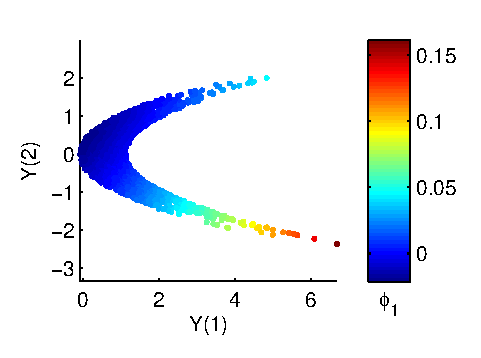
\includegraphics[width=\textwidth]{data_transformed_colored_DMAPS}
%\caption{}
%\end{subfigure}
%\caption{(a) The data from Figure~\ref{fig:initial_data}(b), colored by the first NIV (we take $\sigma_{kernel} = 0.01$, and $\delta t = 10^{-9}$). Note that we recover the slow variable. (b) The data from Figure~\ref{fig:initial_data}(b), colored by the first DMAPS variable (we take $\sigma_{kernel} = 0.01$). Note that we do {\em not} recover the slow variable.}
%\label{fig:NIV_versus_DMAPS}
%\end{figure}

\subsection{Determining Appropriate Parameters}

We would like to demonstrate how we can {\em empirically} determine the appropriate parameters $\delta t$ and $\sigma_{kernel}$ so that we can accurately recover the slow variable(s).

For the system in \eqref{eq:init_data} and \eqref{eq:transformed_data}, the three relevant quantities for NIVs are 
\begin{itemize}
\item The linearized approximation to the distance,
%
\begin{equation}
(Y_2 - Y_1)^T (JJ^T)^{-1} (Y_2 - Y_1) 
\approx \mathcal{O} \left(  \frac{1}{2} \left( 2 + \epsilon + \sqrt{ 9 + 2 \epsilon + \epsilon^2}\right) \Delta Y^2\right) 
\end{equation}
where $\Delta Y =  \|Y_2 - Y_1\|$

\item The error from the {\em estimation} of the covariance.
%
This is
\begin{equation}
\frac{\delta t}{2} (Y_2 - Y_1)^T A (Y_2 - Y_1) \approx \mathcal{O} \left( \frac{38 \delta t}{\epsilon ^2 + 2 \delta t}\Delta Y^2 \right)
\end{equation}

\item The errors from the {\em truncation} of the Taylor expansion for the Mahalanobis distance, which is 
\begin{equation}
n \left( \left| K_1 K_2 \right| + \left| \frac{ K_2^2}{4} \right|  + \left| \frac{K_1 K_3}{3} \right|  \right) \| Y_2 - Y_1 \| ^4 \approx \mathcal{O} \left( 10 \Delta Y^4  \right) 
\end{equation}

\end{itemize}
%
We can plot each of these quantities analytically as a function of $\delta t$ and $\|Y_2 - Y_1\|$. 
%
The results are shown in Figure~\ref{fig:empirical_estimation}(a)~and~(c). 
%
In practice, for more complex SDEs, we cannot write down the three terms analytically.
%
We can only measure the sum of the three terms; this is the estimate of the intrinsic distance that we calculate, $\|X_2 - X_1 \|^2_{est}$.
%
This is also shown in Figure~\ref{fig:empirical_estimation}(a)~and~(c).
%
Clearly, when higher-order terms become important corresponds to a ``kink'' in the plots. 
%
We can also plot the empirical estimates of $\| X_2 - X_1 \|^2_{est}$ obtained from simulation data, as a function of $\delta t$ and $\| Y_2 - Y_1 \|$.
%
This is shown in Figure~\ref{fig:empirical_estimation}(b)~and~(d). 
%
The same ``kink'' is evident in these plots at approximately the same position as the analytical plots. 
%
Therefore, we choose $\delta t$ and a $\sigma_{kernel}$ which corresponds to a $\|X_2 - X_1 \|_{est}^2$ value {\em before} the kink. 
%
For this particular example, we take $\delta t = 10^{-9}$ and $\sigma_{kernel} = 0.01$, which allows us to accurately recover the slow variable. 

%\begin{figure}[h]
%\begin{subfigure}{0.5\textwidth}
%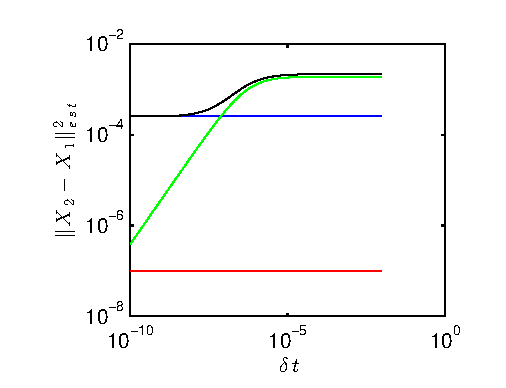
\includegraphics[width=\textwidth]{errors_function_dt}
%\caption{}
%\end{subfigure}
%\begin{subfigure}{0.5\textwidth}
%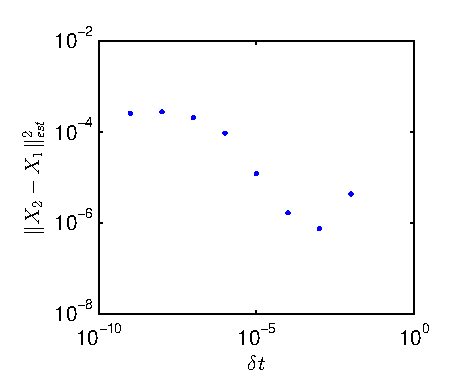
\includegraphics[width=\textwidth]{empirical_totaldist_function_dt}
%\caption{}
%\end{subfigure}
%\begin{subfigure}{0.5\textwidth}
%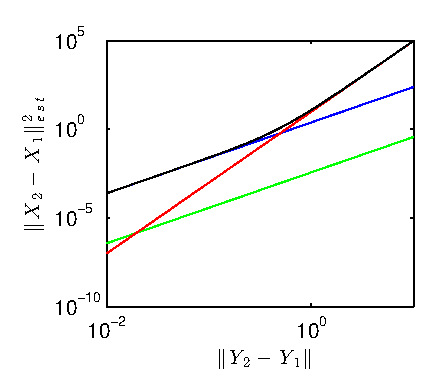
\includegraphics[width=\textwidth]{errors_function_dy}
%\caption{}
%\end{subfigure}
%\begin{subfigure}{0.5\textwidth}
%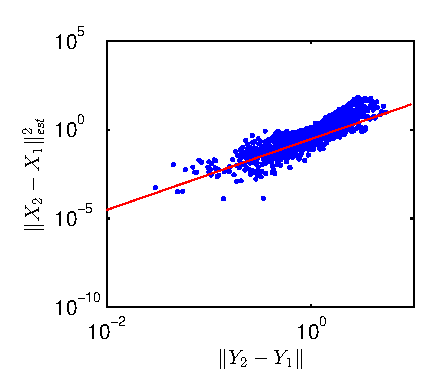
\includegraphics[width=\textwidth]{empirical_totaldist_function_dy}
%\caption{}
%\end{subfigure}
%\caption{(a) Total estimated distance (black) and the three separate terms in the estimated distance, as a function of $\delta t$. The linearized approximation is in blue, the error from the covariance estimation is in green, and the error from the truncation of the distance expansion is in red. 
%%
%(b) Empirical estimation of total distance as a function of $\delta t$, with $\|Y_2 - Y_1 \|^2 = 0.01$.  
%%
%(c) Total estimated distance (black) and the three separate terms in the estimated distance, as a function of $\|Y_2 - Y_1\|$. The linearized approximation is in blue, the error from the covariance estimation is in green, and the error from the truncation of the distance expansion is in red. 
%%
%(d) Empirical estimation of total distance as a function of $\|Y_2 - Y_1\|$, with $\delta t =  10^{-9}$. The red line corresponds to the quadratic $\|X_2 - X_1 \|^2_{est} \propto \|Y_2 - Y_1 \|^2$.}
%\label{fig:empirical_estimation}
%\end{figure}
%
%\begin{figure}
%\begin{subfigure}{0.5\textwidth}
%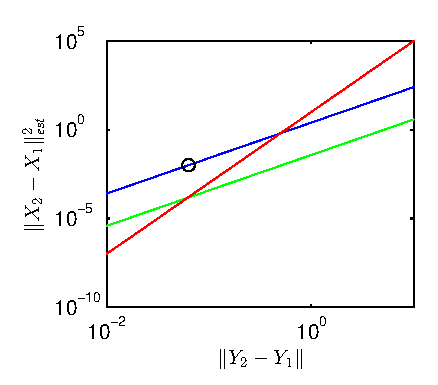
\includegraphics[width=\textwidth]{changing_parameters_error_terms_1}
%\caption{}
%\end{subfigure}
%\begin{subfigure}{0.5\textwidth}
%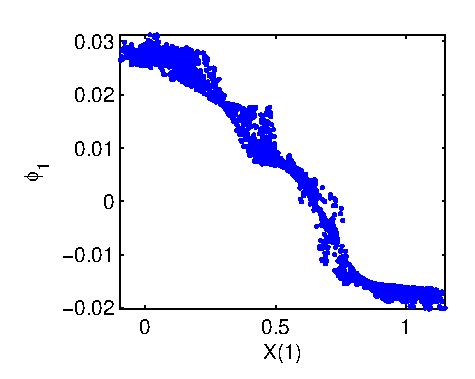
\includegraphics[width=\textwidth]{changing_parameters_NIV_corr_1}
%\caption{}
%\end{subfigure}
%
%\begin{subfigure}{0.5\textwidth}
%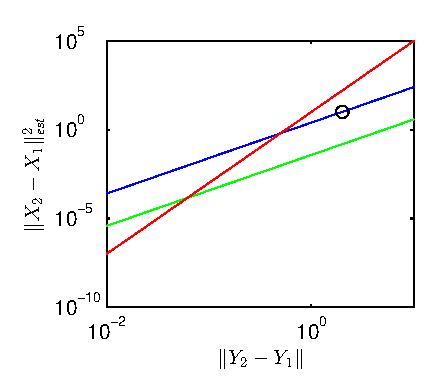
\includegraphics[width=\textwidth]{changing_parameters_error_terms_2}
%\caption{}
%\end{subfigure}
%\begin{subfigure}{0.5\textwidth}
%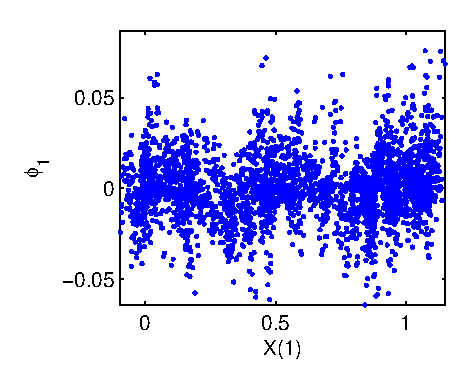
\includegraphics[width=\textwidth]{changing_parameters_NIV_corr_2}
%\caption{}
%\end{subfigure}
%
%\begin{subfigure}{0.5\textwidth}
%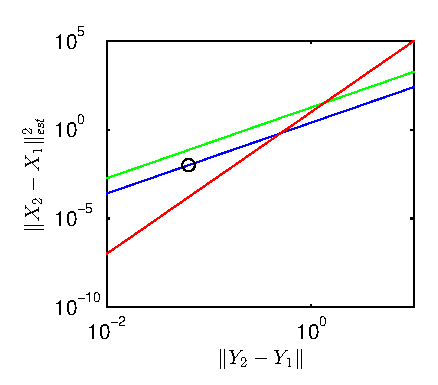
\includegraphics[width=\textwidth]{changing_parameters_error_terms_3}
%\caption{}
%\end{subfigure}
%\begin{subfigure}{0.5\textwidth}
%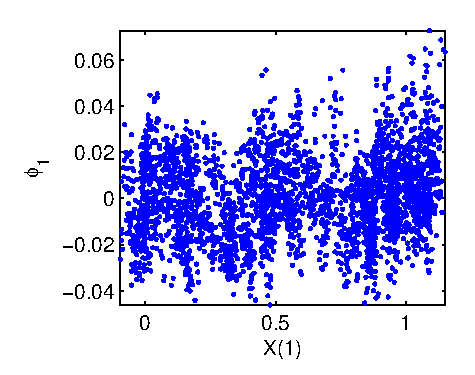
\includegraphics[width=\textwidth]{changing_parameters_NIV_corr_3}
%\caption{}
%\end{subfigure}
%
%\caption{ Error analysis and recovery of the slow variable for three different simulation configurations. (a, b) $\sigma_{kernel} = 10^{-2}$, $\delta t = 10^{-9}$, (c, d) $\sigma_{kernel} = 10^{2}$, $\delta t = 10^{-9}$ (e, f) $\sigma_{kernel} = 10^{-2}$, $\delta t = 10^{-5}$.  (a, c, e) The three separate terms in the estimated distance, as a function of $\|Y_2 - Y_1\|$. The linearized approximation is in blue, the error from the covariance estimation is in green, and the error from the truncation of the distance expansion is in red. The blue circle indicates the value of $\sigma_{kernel}$ used in the diffusion maps calculations. (b, d, f) The first NIV, obtained from the transformed data $Y$, versus the slow variable $X(1)$. Note that we only recover the slow variable $X(1)$ when the linearized approximation dominates the other two error terms in the distance function at the scale of $\sigma_{kernel}$. }
%
%\end{figure}

\subsection{Recovery of Fast Variable}

The size of the ``burst'' we take also affects the recovery of the fast variable, even when there is no nonlinear transformation.
%
When the time scale of the burst is smaller than that of the equilibration time of the fast variable, the estimated covariance is constant and the fast variable is collapsed significantly relative to the slow variable.
%
This means that the fast variable is recovered {\em very} far down in the DMAPS eigenvectors.
%
However, if the time scale of the burst is {\em longer} than the saturation time of the fast variable, the estimated covariance changes: the variance in the slow direction continues to grow, while the variance in the fast direction is fixed.
%
This means that the collapse of the fast variable is less pronounced relative to the slow variable, and the fast variable is recovered in a higher eigenvector. 

We again consider the SDE system from \eqref{eq:init_data}, and consider the transformation
\begin{eqnarray}\label{eq:transformed_data2}
h^1(X) &=& X(1)  \\
h^2(X) &=& \frac{X(2)}{\sqrt{\epsilon}}
\end{eqnarray}
%
Unlike previously, there is no nonlinear component to the transformation, only a rescaling that makes the noise in the ``fast'' direction larger. 

Figure~\ref{fig:vary_burst} shows data collected from simulation of \eqref{eq:transformed_data2}.
%
Different timescales were used to simulate the bursts and estimate the local covariance. 
%
We can see that, when the timescale is less than the saturation time of the fast variable (the first two plots), the fast variable is recovered deep in the eigenvalue spectrum (eigenvector 14).
%
However when the timescale exceeds the saturation time of the fast variable (the third plot), the fast variable moves up in the eigenvalue spectrum (eigenvector 8).

%\begin{figure}[h]
%%\begin{subfigure}{0.5\textwidth}
%%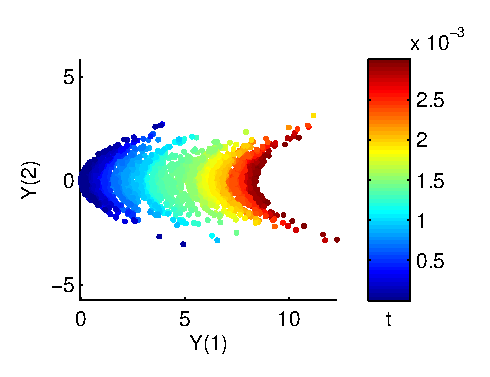
\includegraphics[width=\textwidth]{dat_varyburst}
%%\caption{}
%%\end{subfigure}
%%
%\begin{subfigure}{0.3\textwidth}
%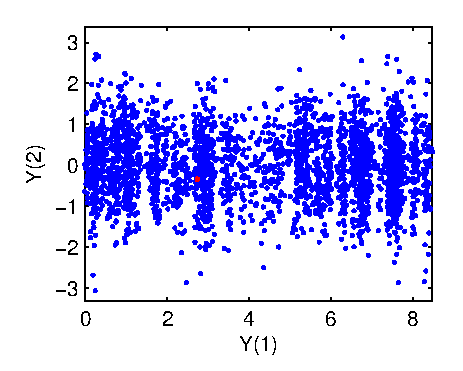
\includegraphics[width=\textwidth]{data_withburst_1}
%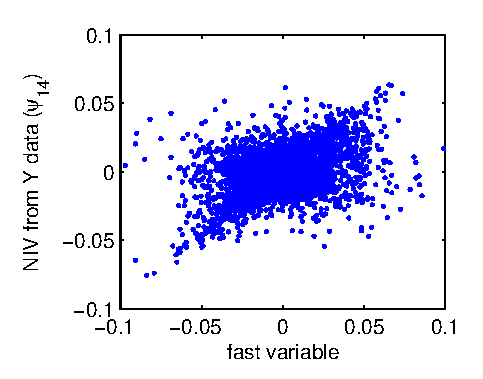
\includegraphics[width=\textwidth]{fast_var_corr_1}
%\caption{}
%\end{subfigure}
%\begin{subfigure}{0.3\textwidth}
%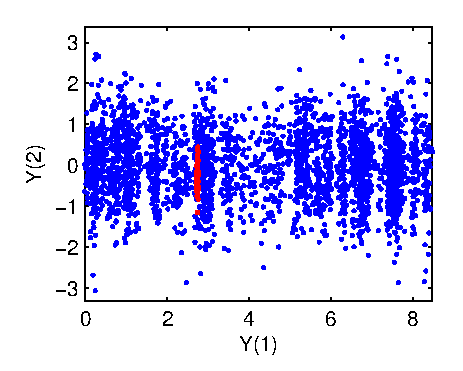
\includegraphics[width=\textwidth]{data_withburst_2}
%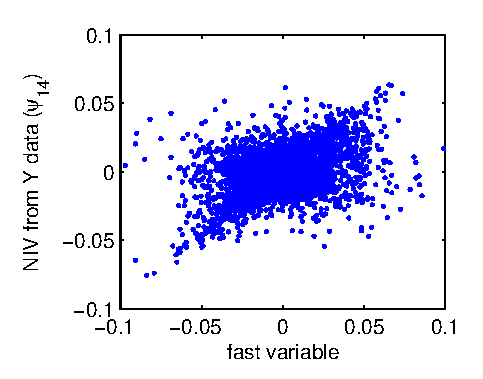
\includegraphics[width=\textwidth]{fast_var_corr_2}
%\caption{}
%\end{subfigure}
%\begin{subfigure}{0.3\textwidth}
%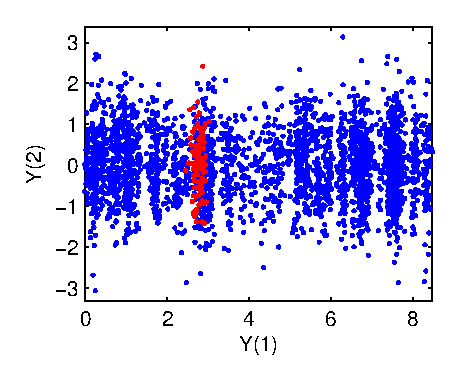
\includegraphics[width=\textwidth]{data_withburst_3}
%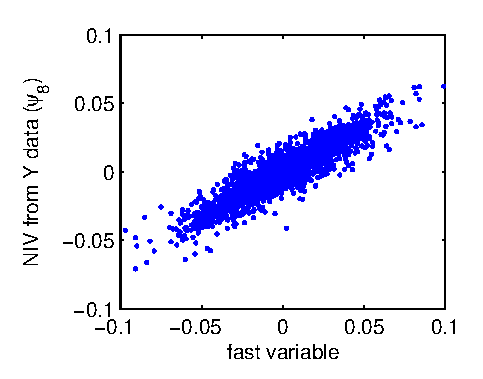
\includegraphics[width=\textwidth]{fast_var_corr_3}
%\caption{}
%\end{subfigure}
%\caption{
%(a) Top: data in blue, simulated from \eqref{eq:init_data} and \eqref{eq:transformed_data2}, with representative burst in red.  
%%
%Bottom: correlation between NIV coordinate and fast variable. 
%%
%(b) Top: data in blue, with representative burst in red.  
%%
%Bottom: correlation between NIV coordinate and fast variable. 
%%
%(c) Top: data in blue, with representative burst in red.  
%%
%Bottom: correlation between NIV coordinate and fast variable. }
%\label{fig:vary_burst}
%\end{figure}

\section{Conclusion}

We showed that in certain cases (when we do {\em not} have a simulator where we can change $\delta t$), the data cannot be processed as-is (we cannot find the right kernel scale given a fixed $\delta t$ such that we can accurately recover the slow variable). 

If the cloud of samples is too big then we can observe the cloud of clouds (and those clouds can be histograms, Fourier, scattering, etc.) as a way to get smaller clouds. 


Richardson extrapolation could allow us to get an estimate of a second-order term in the covariance estimation, thereby locally approximating the function using a quadratic form, rather than a linear form,  which can lead to a better/improved/more accurate ``Mahalanobis'' metric. 


\end{document}
%% end of file `docultexmm.tex'
